\documentclass[12pt,letterpaper]{article}
\usepackage{fullpage}
\usepackage[top=2cm, bottom=4.5cm, left=2cm, right=2cm]{geometry}
\usepackage{amsmath,amsthm,amsfonts,amssymb,amscd}
\usepackage{lastpage}
\usepackage{enumerate}
\usepackage{fancyhdr}
\usepackage{mathrsfs}
\usepackage{xcolor}
\usepackage{graphicx}
\usepackage{listings}
\usepackage{hyperref}
\usepackage{dirtytalk}
\usepackage{tikz}
\usepackage{float}
\usetikzlibrary{automata, positioning, arrows}
\tikzset{
->, % makes the edges directed
>=stealth', % makes the arrow heads bold
node distance=3cm, % specifies the minimum distance between two nodes. Change if necessary.
every state/.style={thick, fill=gray!10}, % sets the properties for each ’state’ node
}
\hypersetup{%
  colorlinks=true,
  linkcolor=blue,
  linkbordercolor={0 0 1}
}
 
\setlength{\parindent}{0.0in}
\setlength{\parskip}{0.05in}


\newcommand\course{ICSI 509}
\newcommand\NetIDa{Ninad Chaudhari}          
\newcommand\NetIDb{NC731749}

\pagestyle{fancyplain}
\headheight 35pt
\lhead{\NetIDa}
\lhead{\NetIDa\\\NetIDb}
\chead{\textbf{\large Complementing a Regular Expression }}
\rhead{nchaudhari@albany.edu\\ \today}
\lfoot{\course}
\cfoot{}
\rfoot{\small\thepage}
\headsep 1.5em

\begin{document}
Let $L$ be a language specified by
a regular expression~$r ~ = ~ (a \cup ab)^*$. The task is to find a regular expression for~$\overline{L}$, the
complement of~$L$. The alphabet $\Sigma$ is~$\{ a, b \}$.

\section*{Method}
We design an NFA for~$r$, convert the NFA to a DFA, flip the accepting and
non-accepting states to take the complement and then generate the regular expression of this
DFA.

\subsection*{Obtaining the NFA}
The NFA for the given example is:

$$
N_1 = (\{q_0,q_1, q_2, q_3\}, \{a,b\}, \delta, q_0, \{q_0\})
$$
where $\delta$ is defined as : 

\begin{tabular}{|l|l|l|l|}
\hline
     & $\varepsilon$ & a        & b        \\\hline
$q_0$ & $\{q_1\}$                   &          &          \\
$q_1$ &                            & $\{q_2\}$ &          \\
$q_2$ & $\{q_0\}$                   &          & $\{q_3\}$ \\
$q_3$ & $\{q_0\}$                   &          &        \\ \hline
\end{tabular}

\begin{figure}[ht]
\centering
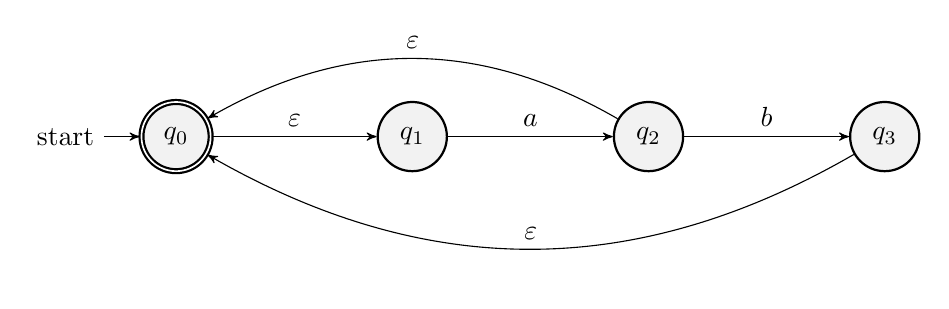
\begin{tikzpicture}
    \node[state, accepting, initial] (q0) {$q_0$};
    \node[state, right of=q0] (q1) {$q_1$};
    \node[state, right of=q1] (q2) {$q_2$};
    \node[state, right of=q2] (q3) {$q_3$};
    
    \draw   (q0) edge[above] node{$\varepsilon$} (q1)
            (q1) edge[above] node{$a$} (q2)
            (q2) edge[above] node{$b$} (q3)
            (q2) edge[above, bend right] node{$\varepsilon$} (q0)
            (q3) edge[above, bend left] node{$\varepsilon$} (q0);
            
\end{tikzpicture}
\caption{NFA for $R$}
\label{fig:nfa}
\end{figure}

Now observe the $\varepsilon$ closures of all states in fig:\ref{fig:nfa}:
\begin{equation}
\label{eq:closure}
\begin{split}
&\varepsilon (q_0) = \{q_0, q_1\} \\
&\varepsilon (q_1) = \{q_1\} \\
&\varepsilon (q_2) = \{q_0, q_1, q_2\} \\
&\varepsilon (q_3) = \{q_0, q_1, q_3\} \\
\end{split}
\end{equation}

\subsection*{Constructing the DFA}
We obtain the DFA by the subset construction method. The states are

\begin{equation}
\begin{split}
    & c_1 = \{q_1, q_2\},\\
    & c_2 = \{q_1, q_2, q_3\},\\
    & c_3 = \{q_1, q_2, q_4\}\\
    & c_4 = \emptyset \\
\end{split}
\end{equation}

\[ 
D_1 = \big( \{c_1, c_2, c_3, c_4\}, \{a,b\}, \delta, c_1, \{c_1, c_2, c_3\} \big)
\]

where $\delta$ is defined as:
\begin{tabular}{|l|l|l|}
\hline
    & a   & b   \\ \hline
$c_1$ & $c_2$ & $c_4$ \\
$c_2$ & $c_2$ & $c_3$ \\
$c_3$ & $c_2$ & $c_4$ \\
$c_4$ & $c_4$ & $c_4$ \\ \hline
\end{tabular}

\begin{figure}[ht]
\centering
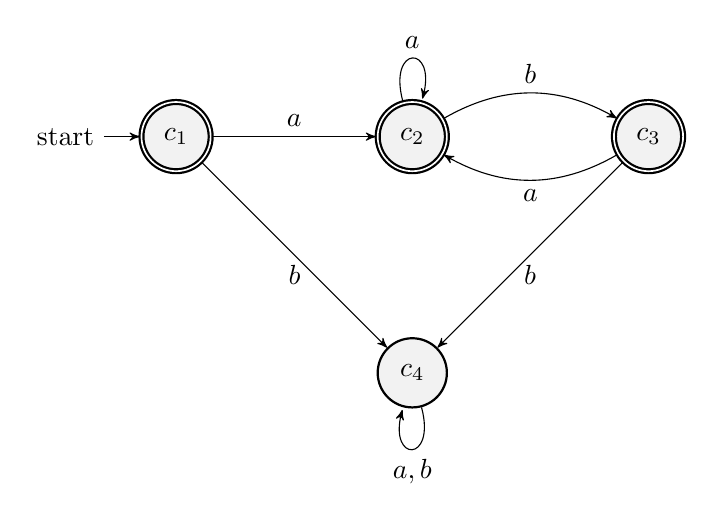
\begin{tikzpicture}
    \node[state, accepting, initial] (q0) {$c_1$};
    \node[state, accepting, right of=q0] (q1) {$c_2$};
    \node[state, accepting, right of=q1] (q2) {$c_3$};
    \node[state, below of=q1] (q3) {$c_4$};
    
    \draw   (q0) edge[above] node{$a$} (q1)
            (q0) edge[below] node{$b$} (q3)
            (q1) edge[loop above] node{$a$} (q1)
            (q1) edge[above, bend left] node {$b$} (q2)
            (q2) edge[below, bend left] node {$a$} (q1)
            (q2) edge[below] node {$b$} (q3)
            (q3) edge[loop below] node{$a,b$} (q3);
            
\end{tikzpicture}
\caption{DFA $D_1$}
\label{fig:dfa}
\end{figure}

% ----------------------------------------------------------------


We can find the complement of the DFA drawn above by flipping the
accepting to non-accepting states and vice-versa. This gives
us the DFA in~Fig~\ref{fig:comp_dfa}

\[ 
D_2 = \big( \{d_1, d_2, d_3, d_4\}, \{a,b\}, \delta, d_1, \{d_4\} \big) \]

where $\delta$ is defined as:
\begin{tabular}{|l|l|l|}
\hline
    & a   & b   \\ \hline
$d_1$ & $d_2$ & $d_4$ \\
$d_2$ & $d_2$ & $d_3$ \\
$d_3$ & $d_2$ & $d_4$ \\
$d_4$ & $d_4$ & $d_4$ \\ \hline
\end{tabular}
\begin{figure}[H] 
\centering
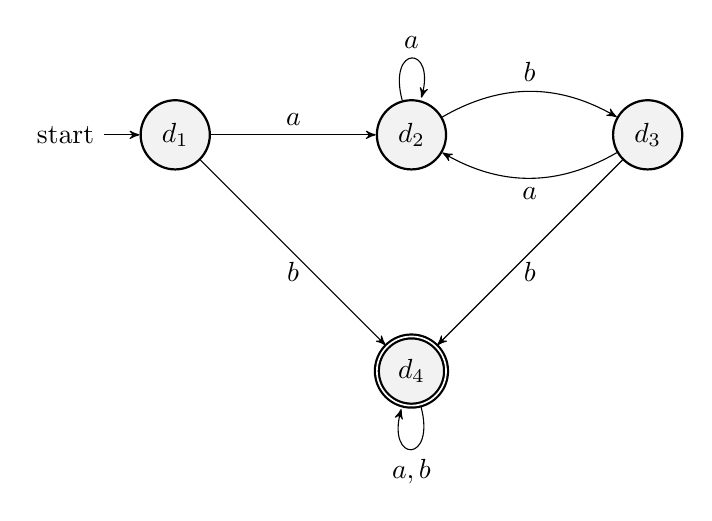
\begin{tikzpicture}
    \node[state, initial] (q0) {$d_1$};
    \node[state, right of=q0] (q1) {$d_2$};
    \node[state, right of=q1] (q2) {$d_3$};
    \node[state, accepting, below of=q1] (q3) {$d_4$};
    
    \draw   (q0) edge[above] node{$a$} (q1)
            (q0) edge[below] node{$b$} (q3)
            (q1) edge[loop above] node{$a$} (q1)
            (q1) edge[above, bend left] node {$b$} (q2)
            (q2) edge[below, bend left] node {$a$} (q1)
            (q2) edge[below] node {$b$} (q3)
            (q3) edge[loop below] node{$a,b$} (q3);
            
\end{tikzpicture}
\caption{Complemented DFA $D_2$}
\label{fig:comp_dfa}
\end{figure}

\subsection*{Obtaining the RegEx}
From the DFA in Fig:\ref{fig:comp_dfa}, we can obtain the following Equations
\begin{equation}
\label{eq:x1}
        X_1 = aX_2 \cup bX_4
        \end{equation}
\begin{equation}
\label{eq:x2}
        X_2 = aX_2 \cup bX_3
        \end{equation}
\begin{equation}
\label{eq:x3}
        X_3 = aX_2 \cup bX_4
        \end{equation}
\begin{equation}
\label{eq:x4}
        X_4 = (a\cup b)X_4 \cup \varepsilon
        \end{equation}
We need to find the regular expression for~$X_1$.

Applying Arden's lemma on equation \ref{eq:x4}, we obtain : 
\begin{equation}
    \label{eq:x4-2}
    X_4 = {(a \cup b)} ^*
\end{equation}
By Arden's lemma, eq:\ref{eq:x3} and the Distributive Law we can transform eq:\ref{eq:x2}:
\begin{equation}
    \label{eq:x2-2}
    \begin{split}
        &X_2 = aX_2 \cup baX_2 \cup bbX_4 \\
        &X_2 = {(a \cup ba)}^* bbX_4\\
    \end{split}
\end{equation}
Now substituting for $X_2$ and $X_4$ we obtain:
\begin{equation}
    X_1 = a{(a \cup ba)}^* bb{(a\cup b)}^* \; \cup \; b(a \cup b )^*
\end{equation}


Hence the regular expression for~$\overline{L}$ is $\; a{(a \cup ba)}^* bb{(a\cup b)}^* \; \cup \; b(a \cup b )^*$
\end{document}
